\documentclass[a4paper,oneside]{memoir}
\usepackage[utf8]{inputenc}
\usepackage{microtype}
\usepackage{graphicx}
\usepackage[linkbordercolor={0.8 0.8 1}]{hyperref} % muss letztes package sein
\title{EasyFlash Application Support}
\author{
Thomas 'skoe' Giesel (skoe@directbox.com) \\
ALeX Kazik
}

\begin{document}
\emergencystretch=0.15\hsize
\maketitle

\tableofcontents

\chapter{Easy File System (EasyFS)}

If you want to store files onto an EasyFlash cartridge, you have to implement a
kind of file system. Easy File System (EasyFS) is a file system which is used
e.g. by the well known EasyLoader.

\section{Introduction}

The original EasyFS specification (EasyFS1) did only store information on how to
launch an entry but doesn't have sufficient information
for determining the exact layout of the cartridge data.
The EasyFS2 specification described in this document addresses this problem and
provides some other improvements, such as more flexibility for PRG file layout.
The differences to the EasyFS1 format are noted for historical purposes.
The name "EasyFS" is used whenever the information is common to both versions.
Newly created tools should use EasyFS2.

This file system is not bound to the EasyFlash hardware or vice versa. It is a
proposal programmers may find useful because there are some tools already which
support it. If you are not familiar with the EasyFlash architecture you should
read EasyFlash-ProgRef.pdf first.

\section{Cartridge Layout}

An example memory layout of an cartridge using EasyFS is shown in \ref{fig:easyfs}.

\begin{figure}[!htbp]
    \centering
    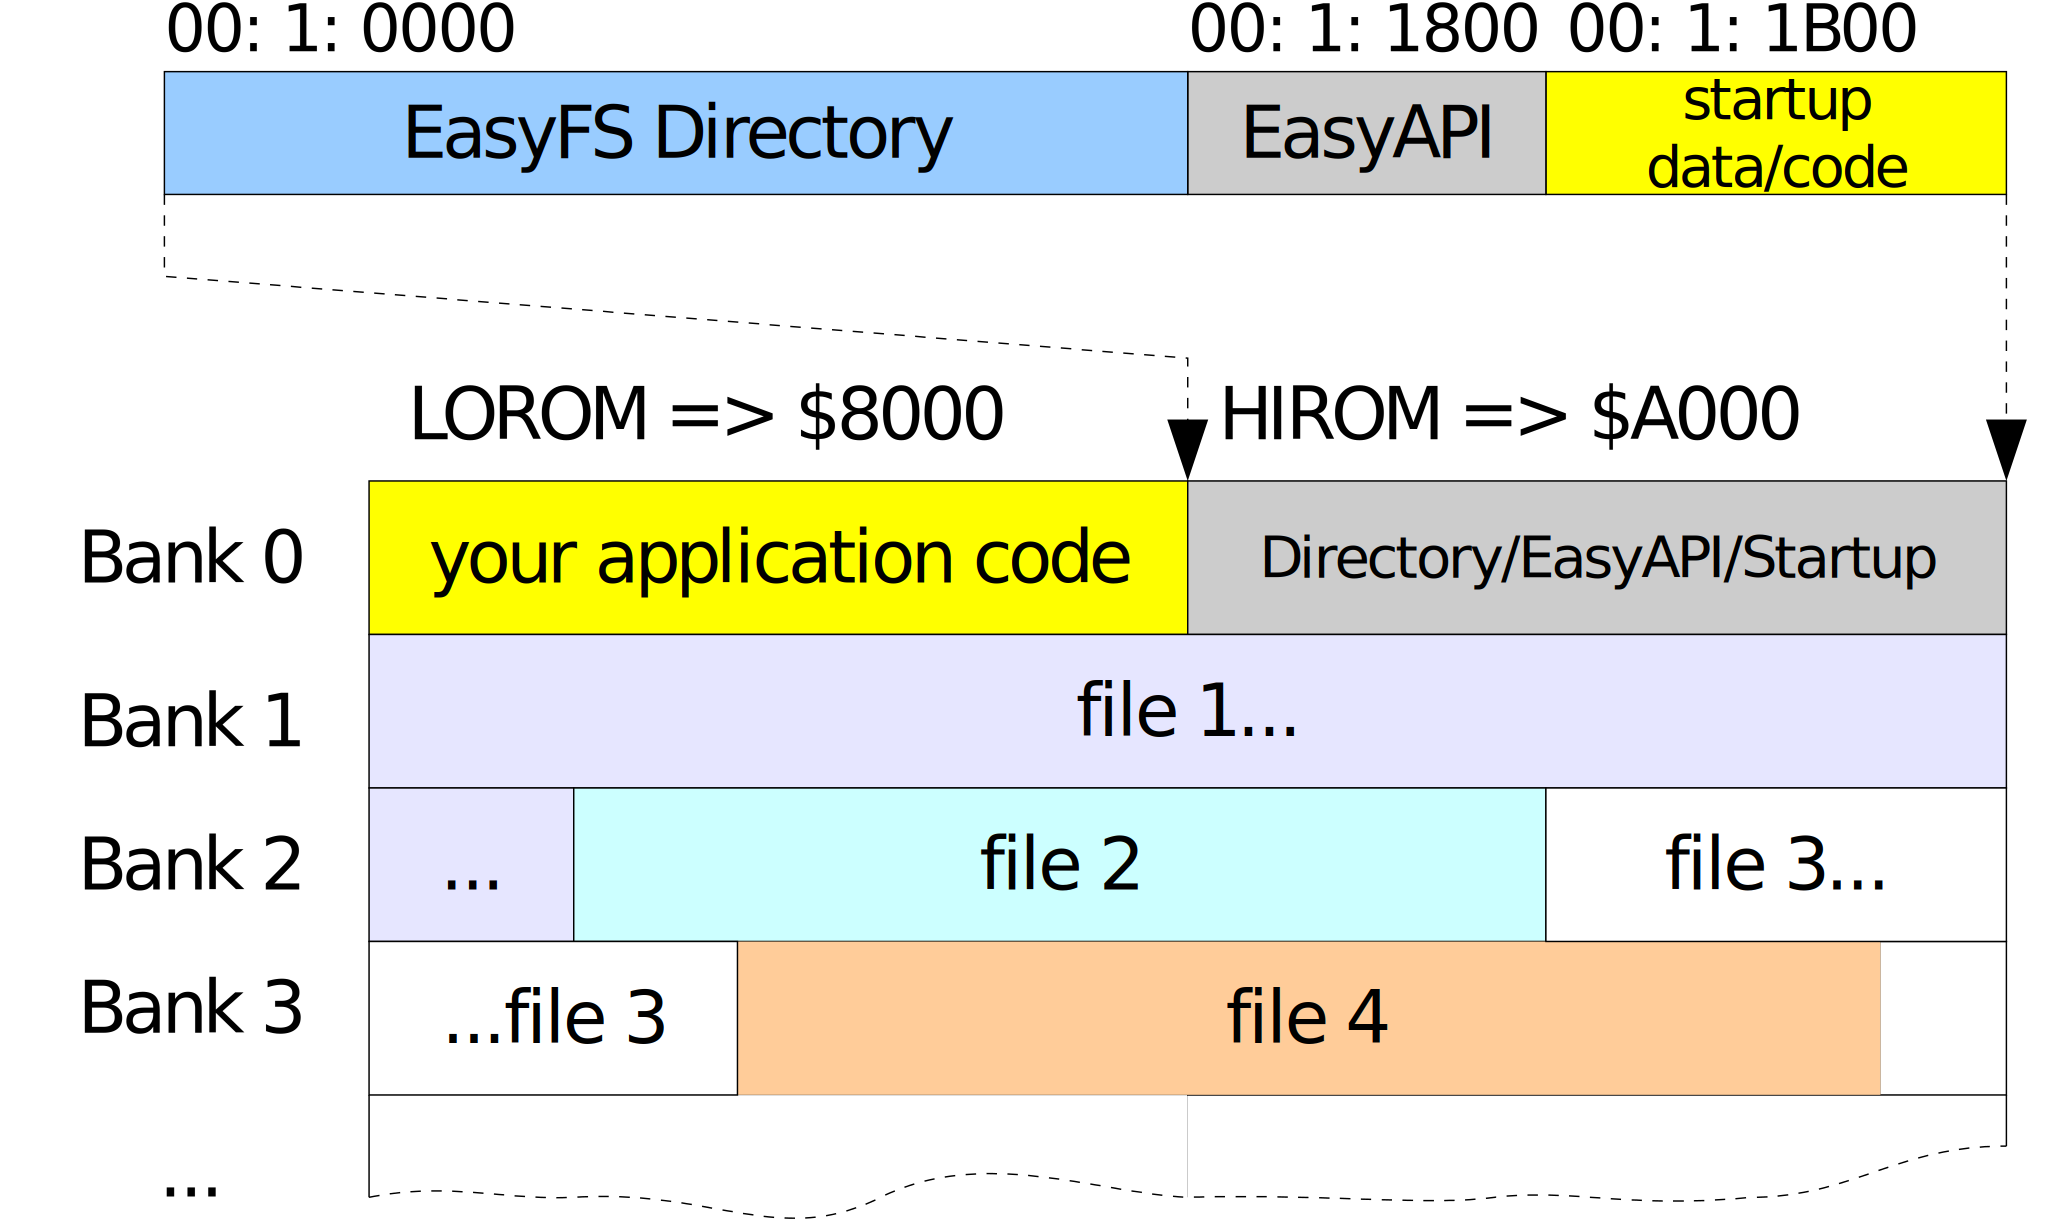
\includegraphics[scale=0.04]{src/easyfs.pdf}
    \caption{EasyFS cartridge layout}
    \label{fig:easyfs}
\end{figure}

Cartridges using EasyFS always use the 16 KiB cartridge mode, which is
configured by the start-up code by setting /GAME and /EXROM active (low). All
explanations in this chapter refer to this configuration.

If your cartridge makes use of the EasyFS, it contains a directory structure.
This structure resides at 00:1:0000. This means it is visible at \$A000 in 16
KiB mode when bank 0 is selected.

A directory shall not contain more than 255 entries (excluding end mark). We
will see that each entry has a size of 24 Bytes, so the whole directory can
have a size of up to \$1800 Bytes. Behind the directory there is space of
\$0800 bytes for EasyAPI and the start-up code and data.

Remember that ROMH is banked in in Ultimax mode at \$E000 after a reset.
Therefore the start-up code contains the reset vector.


\section{Directory Entry}

The directory consists of up to 255 of the following entries (excluding end mark).
Table \ref{tab:easyfs-file-entry} shows the format of EasyFS directory entries.

\begin{table}[!htbp]
    \centering
    \begin{tabularx}{\textwidth}{ ccX }
        \toprule
        Field & Size & Comment \\
        \midrule
        Name              & 16 bytes & File name, 16 characters PETSCII, 0-padded \\[3pt]
        Flags             & 1 byte   & File type and some flags \\[3pt]
        Bank              & 1 byte   & Bank where the file starts, 0..63 \\[3pt]
        Bank High         & 1 byte   & Reserved, always 0 \\[3pt]
        Offset/CrtUsage\footref{fn:fs-changed} & 2 bytes  & For files: start offset in this bank 0..\$3FFF, little endian;
                                       For anything else: see CrtUsage table \ref{tab:easyfs-crtusage}\\[3pt]
        Size              & 3 bytes  & File size, little endian \\[3pt]
        \bottomrule
    \end{tabularx}
    \caption{EasyFS file entry}
    \label{tab:easyfs-file-entry}
\end{table}
\stepcounter{footnote}
\footnotetext{Has a different meaning in EasyFS1\label{fn:fs-changed}}


\subsection{Flags}

Table \ref{tab:easyfs-flags} contains the meaning of the flags field. The bit H
means hidden. If this is 1, this file is not intended to be seen by a user, a
file browser should not show it. Reserved bits marked with R must
\footnote{Unfortunately many tools have ignored this rule.
Encountering a cartridge image that uses 0 for the R bits is likely.}
be set to 1.

\begin{table}[!htbp]
    \centering
    \begin{tabularx}{0.6\textwidth}{X|c|c|c|c|c|c|c|c}
        \toprule
        Bit     & 7 & 6 & 5 & 4 & 3 & 2 & 1 & 0 \\
        \midrule
        Meaning & H & R & R & \multicolumn{5}{c}{Type} \\
        \bottomrule
    \end{tabularx}
    \caption{Flags in EasyFS file entries}
    \label{tab:easyfs-flags}
\end{table}

Table \ref{tab:easyfs-file-types} shows possible values of the Type field.

\begin{table}[!htbp]
    \centering
    \begin{tabularx}{\textwidth}{ cX }
        \toprule
        Field & Type \\
        \midrule
        \$00 & Files with this type are marked as invalid, they must be
        skipped. Note that the flags of this file may be not 0. \\[3pt]
        \$01 & Normal PRG file with 2 bytes start address \\[3pt]
        \$02 & Normal PRG file with 2 bytes start address, only ROML used\footref{fn:fs-new} \\[3pt]
        \$03 & Normal PRG file with 2 bytes start address, only ROMH used\footref{fn:fs-new} \\[3pt]
        \ldots & Reserved \\[3pt]
        \$10 & Normal 8 KiB cartridge (\$8000..\$9FFF) \\[3pt]
        \$11 & Normal 16 KiB cartridge (\$8000..\$9FFF, \$A000..\$BFFF) \\[3pt]
        \$12 & Normal Ultimax cartridge (\$8000..\$9FFF, \$E000..\$FFFF) \\[3pt]
        \$13 & Normal Ultimax cartridge, ROML not used (\$E000..\$FFFF) \\[3pt]
        \$14 & Ocean Type 1, 512 KiB\footref{fn:fs-new} \\[3pt]
        \$15 & Ocean Type 1, 16 KiB to 256 KiB (alternating banks)\footref{fn:fs-new} \\[3pt]
        \ldots & Reserved \\[3pt]
        \$1C & xbank, start in 8 KiB mode, any size\footref{fn:fs-new} \\[3pt]
        \$1D & xbank, start in 16 KiB mode, any size\footref{fn:fs-new} \\[3pt]
        \$1E & xbank, start in Ultimax mode, any size\footref{fn:fs-new} \\[3pt]
        \$1F & End of directory. This entry is only a terminator. \\[3pt]
        \bottomrule
    \end{tabularx}
    \caption{EasyFS file types}
    \label{tab:easyfs-file-types}
\end{table}
\stepcounter{footnote}
\footnotetext{This type is new to EasyFS2\label{fn:fs-new}}

Note that in erased flash memory all bits are 1. This means that an entry
located in erased flash has the type \$1F naturally. Furthermore, when flash is
written, bits can only turn from 1 to 0. It is not possible to change a bit
from 0 to 1 when writing to flash memory. That's why the file type \$00 marks a
deleted or invalid file. \$00 can be written regardless from the old file type
by only changing ones to zeros.

When starting a CRT (type \$10..\$1E) the two lowest bits describe the
mode to start in. The whole information is useful in extracting entries
from an assembled cartridge.


\subsection{Bank}

The EasyFS1 defined the two Bank bytes as 1 byte for Bank and 1 reserved byte, which has to be 0.
With the EasyFS2 it is a 2 byte wide, so all EasyFS1 entries are full compatible.


\subsection{CrtUsage}

Table \ref{tab:easyfs-crtusage} shows the meaning of the CrtUsage field.
Note that this field is EasyFS2 specific. EasyFS1 has this field set to either \$0000 or \$2000
for all cartridge entries (the offset, \$2000 for 8 KiB ultimax cartidges, \$0000 for all others).
This field is only used for entries of type cartridge (Type \$10..\$1E).

\begin{table}[!htbp]
    \centering
    \begin{tabularx}{\textwidth}{ cX }
        \toprule
        Bit & Meaning \\
        \midrule
        15      & Must be 1 \\[3pt]
        14      & 1 if the cartridge should be seen as a subdirectory
                  (only valid for EasyFlash and xbank) \\[3pt]
        13      & 1 if the cartridge must be placed on a 64 KiB boundary
                  (ony valid for xbank) \\[3pt]
        12..8   & Number of banks free at the beginning of the opposite ROM
                  (0..31) \\[3pt]
        7..0    & Number of banks in the opposite ROM
                  (0..255) \\[3pt]
        \bottomrule
    \end{tabularx}
    \caption{EasyFS2 CrtUsage field}
    \label{tab:easyfs-crtusage}
\end{table}

In order to safely extract an entry from an assembled cartridge it's
necessary to know exactly which space it occupies. For files that's easy:
it starts on a specified bank and offset and when it hits the end of a bank
it just continues to the next. For a cartridge it can be more complex.

Table \ref{tab:bank-usage-oc1-256k} shows the usage of the Shadow of the Beast cartridge.
In order to specify which banks are used the use of only Offset and Size is not sufficient.

\begin{table}[!htbp]
    \centering
    \begin{tabularx}{0.6\textwidth}{c|X|X}
        \toprule
        Bank & ROML & ROMH \\
        \midrule
        31 & - & Used \\
        \ldots & - & Used \\
        16 & - & Used \\
        15 & Used & - \\
        \ldots & Used & - \\
        0 & Used & - \\
        \bottomrule
    \end{tabularx}
    \caption{Example Bank Usage (256 KiB Ocean Type 1)}
    \label{tab:bank-usage-oc1-256k}
\end{table}

The "opposite ROM" is the ROM (LO or HI) which does not contain the startup code.
For normal cartridges the startup code is in the ROML, thus the opposite is ROMH.
Ultimax cartiridges on the other hand do have the startup code in ROMH
(making ROML the opposite).

In case of the Shadow of the Beast cartridge
there are 16 banks in the opposite ROM and also 16 banks free at the
beginning of the opposite ROM. Now it's easy to calculate how much of the
"non opposite" ROM is filled: number of total banks (256 KiB / 8 KiB = 32)
minus the banks used in the opposite ROM (16) results in 16 banks.

The opposite ROM is defined as follows:
\begin{itemize}
\item[-] ROMH when Type \& 3 is 0 or 1
\item[-] ROML when Type \& 3 is 2 or 3
\end{itemize}

When bit 15 of CrtUsage (for cartridges) is 0 then this is an old EasyFS1
entry and it's not known which banks this cartridge occupies.
It's unsafe to extract this entry.


\chapter{Supported cartridge types}

Different types of cartridge images can be written to and started from an
EasyFlash cartridge. Let's have find out how these work.

\section{Native EasyFlash Cartridges}\label{native-easyflash-cartridges}

Native EasyFlash Cartridges can use the full flash memory of 1 MiB. They can
use any kind of banking which is supported by the EasyFlash hardware in any way
they want. This is most probably the cartridge format you want to develop for.

EasySDK comes with some tools and code snippets to create, write and read
EasyFlash cartridges.
As already mentioned, EasyFlash cartridges always start in Ultimax mode.
Therefore there is a small boot code required at the end of the ROMH flash chip
on bank 0 (00:1:1xxx). This start-up code is executed directly after a CPU
reset.
The start-up code has to:

\begin{itemize}
  \item Provide the reset vector
  \item Initialize the CPU registers \$01 and \$00 (in this order)
  \item Initialize all I/O you need (SID, VIC-II etc.)
  \item Scan the keyboard
  \item Set up \$DE02 and start the stuff
\end{itemize}

A reference implementation for the start-up code can be found in
examples/banking-test.

If a native EasyFlash CRT wants to write to the flash memory, it may contain a
piece of code called EasyAPI. This is described in EasySDK.pdf.

The memory area from 00:01:1800 to 00:01:1AFF is reserved for EasyAPI. So the
startup code and data can occupy e.g. the area 00:01:1B00 to 00:01:1FFF. A part
of this area may be used to embed a cartridge name, refer to EasySDK.pdf for more information.

\section {Normal 8 KiB Cartridges}

Normal 8 KiB cartridges consist of up to 8 KiB of ROM visible at \$8000 (ROML).
This type of cartridges pulls down /EXROM and leaves /GAME high.
The memory at \$8000 contains some magic bytes. The C64 Kernal detects these
bytes in the reset code. If such a cartridge is found, it gets started with
JMP(\$8000).

EasyFlash cartridges always start in Ultimax mode. Therefore EasyProg adds
start-up code automatically when flashing 8 KiB cartridges.

\section{Normal 16 KiB Cartridges}

Normal 16 KiB cartridges consist of up to 16 KiB of ROM. 8 KiB are visible at
\$8000 (ROML) and 8 KiB at \$A000 (ROMH). This type of cartridges pulls down
/EXROM and /GAME.
The memory at \$8000 contains some magic bytes. The C64 Kernal detects these
bytes in the reset code. If such a cartridge is found, it gets started with
JMP(\$8000).
EasyFlash cartridges always start in Ultimax mode. Therefore EasyProg adds
start-up code automatically when flashing 8 KiB cartridges.

\section{Ultimax Cartridges}

Ultimax cartridges consist of up to 16 KiB of ROM. 8 KiB are visible at \$8000
(ROML) and 8 KiB at \$E000 (ROMH). This type of cartridges pulls down /GAME and
leaves /EXROM high.
The memory at \$e000 contains the reset vector. When the CPU is reset, the
execution starts at the address pointed to by this vector. This kind of
cartridges must initialize the hardware carefully, because there is no KERNAL
doing this for you.
Even for Ultimax Cartridges EasyProg adds start-up code automatically when they
are flashed.

\section{Ocean Cartridges}

Ocean cartridges are banked cartridges. The bank number is written to \$DE00,
like it is done on EasyFlash.
Real Ocean cartridges do always set bit 7 when they write to \$DE00. This bit
is ignored by EasyFlash.

Ocean cartridges with up to 256 KiB use following banking scheme:

Up to 16 Banks are put to ROML. This means that banks number 0..15 can be found
at ROML. If needed, banks 16..31 are put to ROMH. These cartridges pull down
/EXROM and /GAME, so 16 KiB of ROM are mapped into the C64 memory at once, 8
KiB at \$8000 and 8 KiB at \$A000.
When banks 0..15 are used, which are read from ROML, the content of ROMH is not
used. When banks 16..31 are used, which are read at ROMH, the content of ROML
is not used. This means although 16 KiB are banked in at once, one 8 KiB of
each bank are actually used.

A CRT image only contains the banks actually used.

Example 1: A 128 KiB Ocean cartridge looks like this ('P' = Data, '/' =
undefined / don't care, '-' = nothing):

\small
\begin{verbatim}
BANK  0 0 0 0 0 0 0 0 0 0 0 0 0 0 0 0 1 1 1 1 1 1 1 1 1 1 1 1 1 1 1 1
      0 1 2 3 4 5 6 7 8 9 A B C D E F 0 1 2 3 4 5 6 7 8 9 A B C D E F

ROML  P P P P P P P P P P P P P P P P - - - - - - - - - - - - - - - -
ROMH  / / / / / / / / / / / / / / / / - - - - - - - - - - - - - - - -
\end{verbatim}
\normalsize

Example 2: A 256 KiB Ocean cartridge looks like this:

\small
\begin{verbatim}
BANK  0 0 0 0 0 0 0 0 0 0 0 0 0 0 0 0 1 1 1 1 1 1 1 1 1 1 1 1 1 1 1 1
      0 1 2 3 4 5 6 7 8 9 A B C D E F 0 1 2 3 4 5 6 7 8 9 A B C D E F

ROML  P P P P P P P P P P P P P P P P / / / / / / / / / / / / / / / /
ROMH  / / / / / / / / / / / / / / / / P P P P P P P P P P P P P P P P
\end{verbatim}
\normalsize

There is a completely different type of Ocean cartridge, the 512 KiB type
(Terminator II):

This type also uses \$DE00 for banking. It uses 64 banks of 8 KiB each. All
banks are read from 8 KiB of ROM visible at \$8000 (ROML). This type of
cartridges pulls down /EXROM and leaves /GAME high.

Example 3: A 512 KiB Ocean cartridge looks like this:

\footnotesize
\begin{verbatim}
BANK  0 0 0 0 0 0 0 0 0 0 0 0 0 0 0 0 1 1 1 1 1 1 1 1 1 1 1 1 1 1 1 2 ... 3 3
      0 1 2 3 4 5 6 7 8 9 A B C D E F 0 1 2 3 4 5 6 7 8 9 A B C D E 0 ... E F

ROML  P P P P P P P P P P P P P P P P P P P P P P P P P P P P P P P P ... P P
\end{verbatim}
\normalsize

Ocean cartridge have the advantage to be also compatible to older emulators. On
the other hand the format is not very intuitive.

EasyFlash cartridges always start in Ultimax mode. Therefore EasyProg adds
start-up code automatically when flashing Ocean cartridges.


\chapter{EasyFlash xbank Cartridges}

The EasyFlash xbank cartridge format is a multi-bank cartridge format which can
be placed at any bank in the flash, though all the banks must be continuous.
This makes it possible to combine several xbank cartridges into one cartridge.

Unlike other cartridge types wrapped into *.CRT files this one does not
represent a physical cartridge. Nevertheless the CRT container format is used
for it. The format is similar to the EasyFlash cartridge format. The main
difference is that it can be placed on any bank, unlike EasyFlash or e.g. Ocean
Type 1 cartridges. This makes it possible to have more than one multibank
cartridge on a single EasyFlash.

The GAME and EXROM configuration in the CRT header will be used to determine
which mode should be set at start-up. This is done by the start-up code. This
code will also write the right start bank to \$DE00 and start the cartridge
using the CPU Reset Vector.

The start bank will also be stored in \$DF00 and the program has to care itself
for the addition of the relative bank and the offset before writing it into the
banking register.

EasyProg adds start-up code automatically when flashing an xbank cartridge
directly. Currently EasyProg does not automatically replace/patch EasyAPI for
xbank cartridges.

The magic cartridge id is 33 (\$21).

\end{document}

